\documentclass{article}
\usepackage[UTF8]{ctex}
\usepackage{geometry}
\usepackage{natbib}
\geometry{left=3.18cm,right=3.18cm,top=2.54cm,bottom=2.54cm}
\usepackage{graphicx}
\pagestyle{plain}	
\usepackage{setspace}
\usepackage{caption2}
\usepackage{datetime} %日期
\renewcommand{\today}{\number\year 年 \number\month 月 \number\day 日}
\renewcommand{\captionlabelfont}{\small}
\renewcommand{\captionfont}{\small}
\begin{document}

\begin{figure}
    \centering
    
\includegraphics[width=8cm]{upc.png}

    \label{figupc}
\end{figure}

	\begin{center}
		\quad \\
		\quad \\
		\heiti \fontsize{45}{17} \quad \quad \quad 
		\vskip 1.5cm
		\heiti \zihao{2} 《计算科学导论》课程总结报告
	\end{center}
	\vskip 2.0cm
		
	\begin{quotation}
% 	\begin{center}
		\doublespacing
		
        \zihao{4}\par\setlength\parindent{7em}
		\quad 

		学生姓名:\underline{\qquad  汪子霄 \qquad \qquad}

		学\hspace{0.61cm} 号:\underline{\qquad 1907010222\qquad}
		
		专业班级:\underline{\qquad 计科1902 \qquad  }
		
        学\hspace{0.61cm} 院:\underline{计算机科学与技术学院}
% 	\end{center}
		\vskip 2cm
		\centering
		\begin{table}[h]
            \centering 
            \zihao{4}
            \begin{tabular}{|c|c|c|c|c|c|c|}
            % 这里的rl 与表格对应可以看到,姓名是r,右对齐的;学号是l,左对齐的;若想居中,使用c关键字。
                \hline
                课程认识 & 问题思 考 & 格式规范  & IT工具  & Latex附加  & 总分 & 评阅教师 \\
                30\% & 30\% & 20\% & 20\% & 10\% &  &  \\
                \hline
                 & & & & & &\\
                & & & & & &\\
                \hline
            \end{tabular}
        \end{table}
		\vskip 2cm
		\today
	\end{quotation}

\thispagestyle{empty}
\newpage
\setcounter{page}{1}
% 在这之前是封面,在这之后是正文
\section{引言}
光阴似箭,转眼间,大学第一学期的生活已经结束,计算科学导论在这过程中也已经圆满结束。起初,由于我对计算科学了解甚少,也不知道如何开始学习,但孙运雷老师的循循善诱,使得计算科学在我脑海里渐渐有了一定的认识,它的意义也逐渐清晰。孙老师不仅重视教学,更注意引导我们正确学习,让我们注重团队合作与规划,引导我们寻找正确的人生方向。\par
只有认识世界,才能改变世界,对计算科学也是,这门课程不但在学校学习中起到了一定的启蒙作用,而且对我们认识社会有着启示作用。\par


\section{对计算科学导论这门课程的认识、体会}
不同于大学内其他课程,计算科学导论本身不属于重点课程的范畴,但他对于初学者非常重要,尤其是对于计算机小白的初步引入更是有着举足轻重的作用。这不仅是因为它按照学科系列教材一体化设计的要求,有条不紊地介绍了计算科学的定义、特点、形态、历史渊源、发展变化的知识组织结构和分类体系,学科专业培养模式和课程体系等内容,更因为他通俗流畅的语言文字,深入浅出的描述和严谨的构思设计让大学一年级新生比较全面地了解计算科学,认识并学习计算科学,这类似旅游中对“导游图”的学习和了解。\par
孙老师也布置了相关与课程又急需新生所作的作业任务,进一步帮助我们构造自己的学习框架,从而使我们大学褪去空虚与荒废,引导我们研究与探索课程外的新知识。\par
只有认识世界,才能改造世界。在我看来,计算科学导论是一个认识计算科学的过程,在学习这门课程之后,我发现计算机起源于数学,更有自己的发展道路,也值得我们继续深入研究。\par

\subsection{计算机的数学起源}
在《计算科学导论》第一章中,我们首先接触到计算机的数学起源——从丢番图方程,到费马大定理、无理数和超越数,继而出现的第三次数学危机,然后引出的可计算问题。这些数学问题人们对数学问题的深入思考,是对存在结论的敢于质疑。\par
像提出世界上只有整数和分数(有理数)的毕达哥拉斯,他的得意门生希帕索斯发现2不能通约,不是有理数,这一数学危机持续到世纪下半叶。也正因如此,实数理论建立到更严格的科学基础上。到第三次数学危机罗素悖论打击当时的集合论,知道冯诺依曼提出全体集合构成的集合,不能是集合论的一个对象、元素使罗素悖论“不再存在”。\par
然后希尔伯特计划的出现说明如果集合论是无矛盾的并且所有集合论的命题(从而所有的数学命题)都能从集合论的公理按逻辑演绎的法则推导出来正确,任何数学命题,要知道真假,所要做的不过是从几条公理出发,按逻辑演绎法则去推,总会证明他的真或否,由此说明数学本质上是机械的。而哥德尔不完备定理提出:计算机从根本上说,就是一种基于二进制数字运算的命题演算系统。其中给出的加减法运算公理是有限的,可推到的,可证明的,规则是可计算,也就是说具备一致性。如该定理所言,系统并不完备,于是许多数学家试图将可计算性理论形式化,为计算建立一个数学模型——计算模型,然后从图灵创造了一种通过操作纸带上的符号进行计算的机器理论模型(图灵机),最终到以冯·诺依曼为代表的一批科学家的努力下,确定了现代存储程序式电子数字计算机的基本结构与工作原理。\par
从数学到计算科学,这是科学的一次改革,也是课程的顺利过渡,这让对数学感兴趣的我,对计算科学焕发更热烈的兴趣。\par

\subsection{计算机网络与通信}
随着课程的一步步深入,书中出现的知识的海洋愈发庞大,知识的体系也愈发深刻、清晰。在书中第二章讲到计算机网络与通信,这个更是激起了我的好奇心。\par
信息革命后,随着计算科学及其应用的高速发展,对软硬件和信息资源共享的需求和一大类问题本身具有地域上分布的特点,促进了计算机网络的发展。\par
计算机网络是指是由通信设备和通信线路将一组地理上分布相同(同质)或不同(异质)的计算机、终端及其附属设备按照某种方式互连起来得到的一个计算机硬件系统,也叫网络计算机。在这种计算机硬件系统的基础上,通过开发能协调各台计算机系统工作的通信系统或更进一步的网络操作系统,就能使一组计算机实现软硬件资源共享、协同计算,合作求解一个问题。由这种通信系统或网络操作系统联通网络计算机一起,顺其自然的形成了网络计算机系统。\par

\begin{figure}[h!]
	\centering
	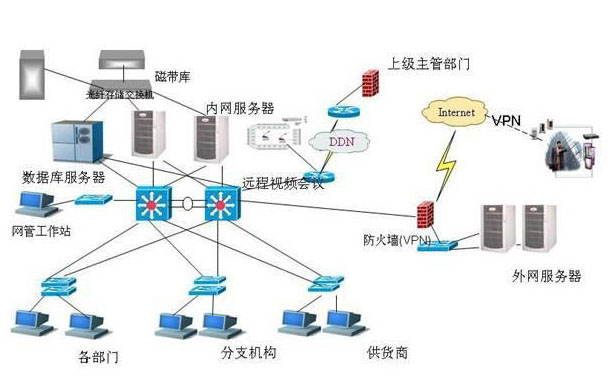
\includegraphics[scale=0.7]{Computer_network}
	\caption{The Computer network}
	\label{fig:Computer_network}
\end{figure}

通信是支持计算机网络的重要技术,它用来实现计算机之间信息传输的技术通信。通信中通信协议是为了在网络计算机系统中实现可靠的、高效的数据交换、差错控制、信息编码、线路利用、同步是通信数据具有透明性。也因为网络通信许多操作十分复杂,网络协议层应运而生。每一层包含一组通信功能和相应的层间通信协议,支持通信双方在不同的层间进行通信,并提供了实现通信的具体思想和方法。按照ISO的建议,网络结构模型是开放系统互联模型OSI(七层协议),包括物理层、数据链路层、网络层、传输层、会话层、表示层、应用层共七层。\par
孙老师的精心准备与赵老师的教材编写双管齐下,使得书中的知识全面且能够把握住着我们的兴趣,让我们持续向下获取新知识。而信息安全领域,更是令我大开眼界,也同时引发了如何保障运输中安全的思考。\par

\subsection{计算机网络通信安全问题}
基于对网络信息安全的好奇,我查阅了期刊《新形式下计算机网络通信中存在的问题及改进策略》\citep{A}希望得到一定的启示。\par
计算机通信高速发展,人们在现代信息社会中的需求不断增加,对于网络通讯的要求越来越高,方便、高速、安全成为了现代网络通信技术发展的必要前提。随着技术的发展,网络通信不仅便利了人们的生活,其中出现的问题也越来越多,计算机网络安全问题也逐渐增加,例如信息泄露问题、黑客问题、网络信号问题,威胁到网络用户的信息安全和用户的使用感受。\par
当前形势下,网络通信主要存在信号强度不足与安全问题。为了更清楚地认识安全中的保障措施,我阅读了期刊《计算机网络通信安全中数据加密技术的应用》\citep{B}。我发现我们应更好的做好网络通信安全管理工作。在当前网络通讯的过程中,确保网络信息安全技术的可靠性最为重要,做好网络通讯的信息管理工作,首先就要实现对网络信息技术的加密,保证信息的可靠安全。现今网络发展过程中最主要的问题,不仅要保证密码算法可以实现数字鉴别、数字加密的功能,还应该把安全保障的目光投放到信息产品安全和管理技术安全上面来,用好的安全管理技术减少黑客和不法分子的攻击,减少人为造成的损失,及时解决面临的安全问题,给人们的生活带来充分的安全和便利。\par
快捷的网络生活逐渐给我们的生活带来了诸多的便利,从最开始2G时代到紧接着的3G时代,到现在我们正在使用的4G,以及华为领先研发的5G的预备应用无不相关着信息安全。\par


\section{进一步的思考}
经过多节课程的学习后,我接触到了计算机的起源,计算机网络与通信安全,这都是与我们生活息息相关的内容。而且,在实际生活中,电脑融于每个人的家庭,手机也早已经普及,那么他们携带的信息又该怎样保护呢?\par
在我留有疑问又不知方向的时候,孙老师为我们提供了六百多种演讲题目,这不仅是课程的一部分,更是老师为我们未来发展方向提供的帮助,基于我内心的疑惑,我找到了同我志同道合的搭档罗胜瀚,在分组演讲中,我们选择了渗透测试的方向。\par

\subsection{网络安全现状}
随着计算机技术的飞速发展,信息网络已经成为社会发展的重要保证。有很多是敏感信息,甚至是国家机密。所以难免会吸引来自世界各地的各种人为攻击(例如信息泄漏、信息窃取、数据篡改、数据删添、计算机病毒等)。同时,网络实体还要经受诸如水灾、火灾、地震、电磁辐射等方面的考验\citep{C}。\par
早在2012年02月04日,黑客集团Anonymous公布了一份来自1月17日美国FBI和英国伦敦警察厅的工作通话录音,时长17分钟,主要内容是双方讨论如何寻找证据和逮捕Anonymous,LulzSec,Antisec,CSL Security等黑帽子黑客的方式\citep{C}。而国内在2011年12月21日,国内知名程序员网站CSDN遭到黑客攻击,大量用户数据库被公布在互联网上,600多万个明文的注册邮箱被迫裸奔。\par
如今中美两国贸易摩擦,就不得不引起我们相关中美网络安全实力的思考。美国是互联网技术最主要的发源地,也是互联网应用最为普及、对网络依赖性很高的国家,网络安全问题成为美国主要现实隐患之一。为维护网络空间安全,美国积极打造网络安全保障体系,并在其国策中突出强调信息安全的重要地位,力图利用网络空间带来的新发展机遇,繁荣经济和推动国家发展,以实力保安全、以安全保发展成为世界网络与信息安全发展大势。与此同时我国正在努力建设网络强国,亟待一个完善的网络信息安全政策体系作为强有力的支撑。2014年我国成立中央网络安全和信息化领导小组,由中央网信办落实中央精神统抓协管、大刀阔斧开展工作,从顶层设计、战略制定、法规完善、科学管理、强化自主可控、开展国际合作等方面大步向前推进,国家网络信息安全政策不断完善,网络与信息安全中的各项工作得到长足推进。国家也将网络安全列为一级学科以培养网络安全人才。\par
\begin{figure}[h!]
	\centering
	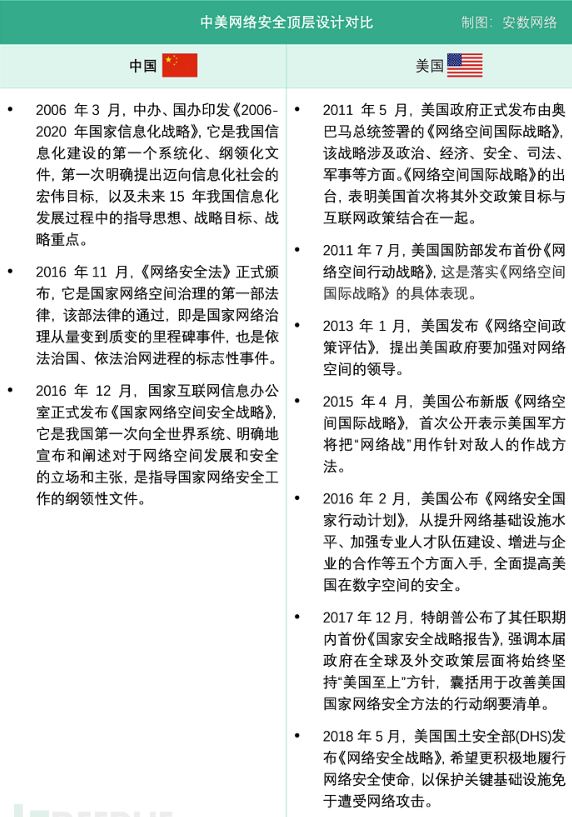
\includegraphics[scale=0.55]{ChUSA}
	\caption{中美顶层设计对比}
	\label{fig:ChUSA}
\end{figure}
在2018年据Cybersecurity Ventures发布的2018全球网络安全企业500强名单,美国有358家上榜,中国8家(乐天,奇虎360,安恒信息,Nexusguard,瀚思,绿盟,深信服,微步在线)上榜。但到2019年,华为苏宁挤进500强20名,这是中华企业的崛起,也是中国实力的提升,相信以华为为代表的一系列中华有为的企业都将在新一年里继续进步,以保障中国安全。\par

\subsection{网络安全的发展趋势}
在网络安全的继续理解过程中,我阅读了期刊《5 G技术对网络空间安全的影响——兼论中美5G竞争》 \citep{20195G},5G的能力在数据传输上是新台阶的突破,它也必将成为中美竞争的新的方向。\par
不同于历史上的第一次第二次工业革命,如今的5G,由中国的华为引领,这是企业的骄傲,更是民族的骄傲。我阅读了《 Network defense and countermeasures: principles and practices》 \citep{Easttom2005Network},在此过程中,我更加理解习主席提出建设网络安全的重要性与华为推出鸿蒙系统的重要意义。

\subsection{渗透测试的发展趋势}
渗透测试是为了证明网络防御按照预期计划正常运行而提供的一种机制。在网络安全的探索过程中,我查阅到图文《Meeting people via WiFi and Bluetooth : mobile security and privacy : advances, challenges and future research directions.
》\citep{RokachMobile},如今Wifi的发展,移动手机端的普及,使得渗透测试从web端渐渐转移至手机端。\par
我阅读了《 Andoroid系统的渗透测试综合平台研究》 \citep{2018Android}手机的渗透测试可以分为3点:\par

\begin{itemize}
	\item 同Web安全渗透测试类似,需要对Server API和终端应用进行安全测试。 
	\item OS本身的特性或安全问题
	\item 应用被逆向破解,业务逻辑和信息被盗取
\end{itemize}
第一块,很多做移动开发的工程师并不一定有Web安全的经验。很多App都存在各种逻辑漏洞,比如App的流程依赖于响应内容且没有做校验。这一类的问题可以通过代理工具进行测试;同样,很多应用对应的服务器也会有一些安全风险点,内部服务开放也可以是渗透的点;\par
第二块会有一些通用的漏洞,比如android老版本的webview代码执行,调试模式的一些安全问题;也会有一些开发习惯的问题,比如SSL证书配置的问题,SQL本地注入和日志信息泄露的问题等。综合来讲,第二块涉及的问题和手机系统本身有很大关联,渗透测试过程中需要不断的积累知识库;\par
第三块是非常重要的,很多时候我们的一些重要业务逻辑会在应用中,如果被黑客或者竞争对手逆向破解,很可能导致商秘泄露或者破解版本的盛行等,导致业务发展受阻。\par

总结起来,前两点通过自己渗透测试或者寻者渗透测试服务能够解决绝大部分风险;最后一点比较复杂,自己实施的话建议业务注意前后端逻辑和关键业务逻辑充分分离,不过通常甲方安全工程师很难保证(业务逻辑性和人力审核成本),简单高效的方式就是购买加固服务。利益相关:网易云易盾提供业内独特的App渗透测试服务(可免费试用),以攻击者的视角,模拟黑客攻击过程,对App(Android、iOS)客户端以及服务端进行深入探测,找出应用系统中存在的缺陷和漏洞,及早发现,及早预防。\par
整个测试过程分为四步:\par
\begin{itemize}
	\item 方案设计:确定渗透测试的时间、方法、测试范围、应急预案等,对整个过程进行监控;
	\item 信息收集:收集网络拓扑结构,对目标系统进行分析,扫描探测,服务查点,查找系统IP等;
	\item 扫描渗透:综合收集的情报,借助工具找到目标系统漏洞,进行渗透入侵,从而获得管理权限;
	\item 检测报告:测试人员根据测试结果,输出渗透测试服务报告。内容包括安全状况、修复建议等。
\end{itemize}

\section{总结}
总的来说,整个课程的学习让我受益匪浅。在孙老师那淳淳的教导下,我不仅了解到计算机的历史起源,这是深入学习计算机的良好启动力,而且,我在孙老师的引导下,我的学习方式从源于老师转变为自主搜索、阅读、学习期刊与图书。更是了解到网络信息安全的一系列知识,从而认识到现今中美贸易战的网络中的竞争问题。\par
如今计算机科学的研究更需队伍协作,而孙老师更是为了培养我们的组队能力,同时老师也注意到团队的整体质量,只要求两个人,我相信这更是在进一步锻炼我们的个人能力。\par
孙老师的课堂也会向我们时刻展现出爱国爱家的思想,同时会向我们普及如今优秀的中国企业,例如:华为,阿里等。我们大一学生有优秀的前辈,我们有明确的方向,这个社会也值得我们为之付出努力。\par

\section{附录}
\subsection{Github账户}
https://github.com/Aptal \par
\begin{figure}[h!]
	\centering
    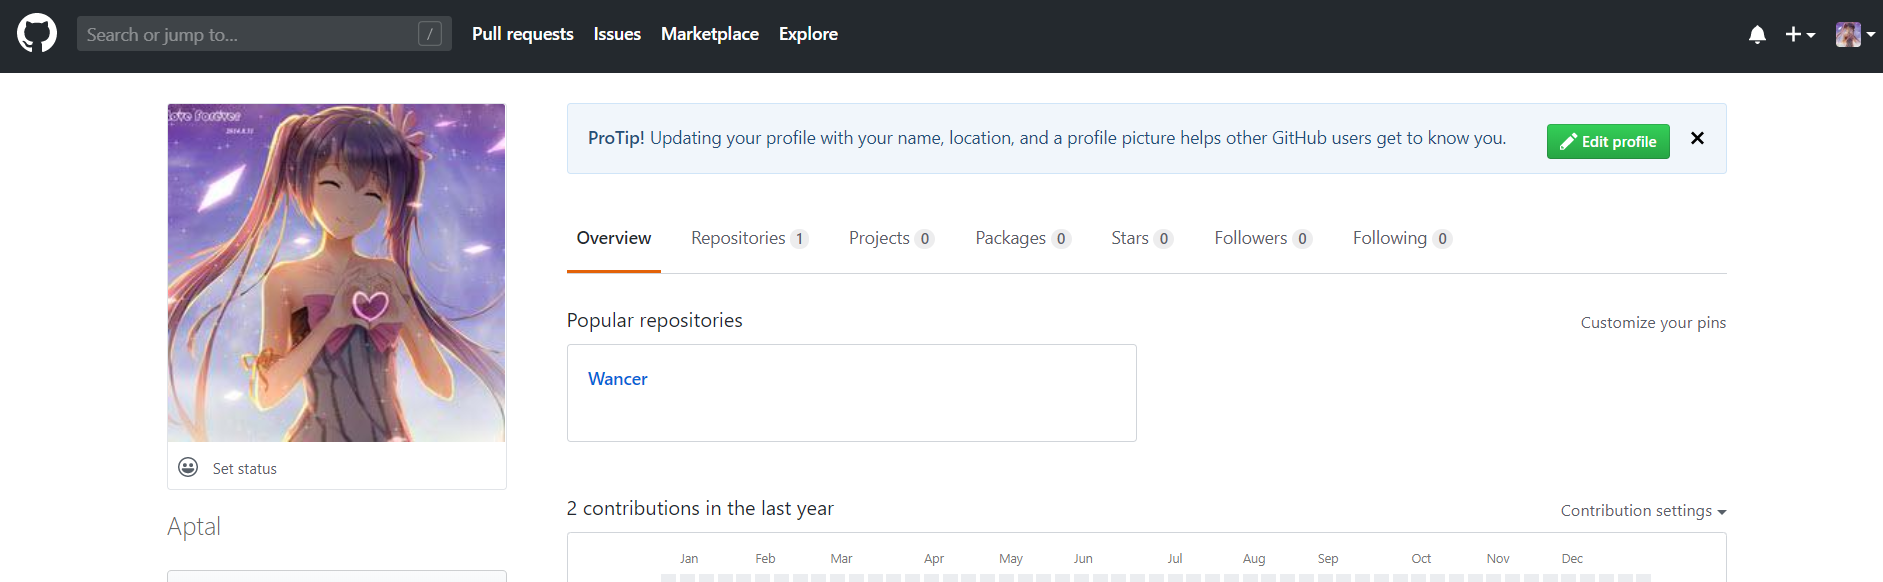
\includegraphics[scale=0.2]{Github}
    \caption{Github账户}
    \label{fig:Github}
\end{figure}

\subsection{CSDN账户}
https://blog.csdn.net/qq\_37572857\par
\begin{figure}[h!]
	\centering
	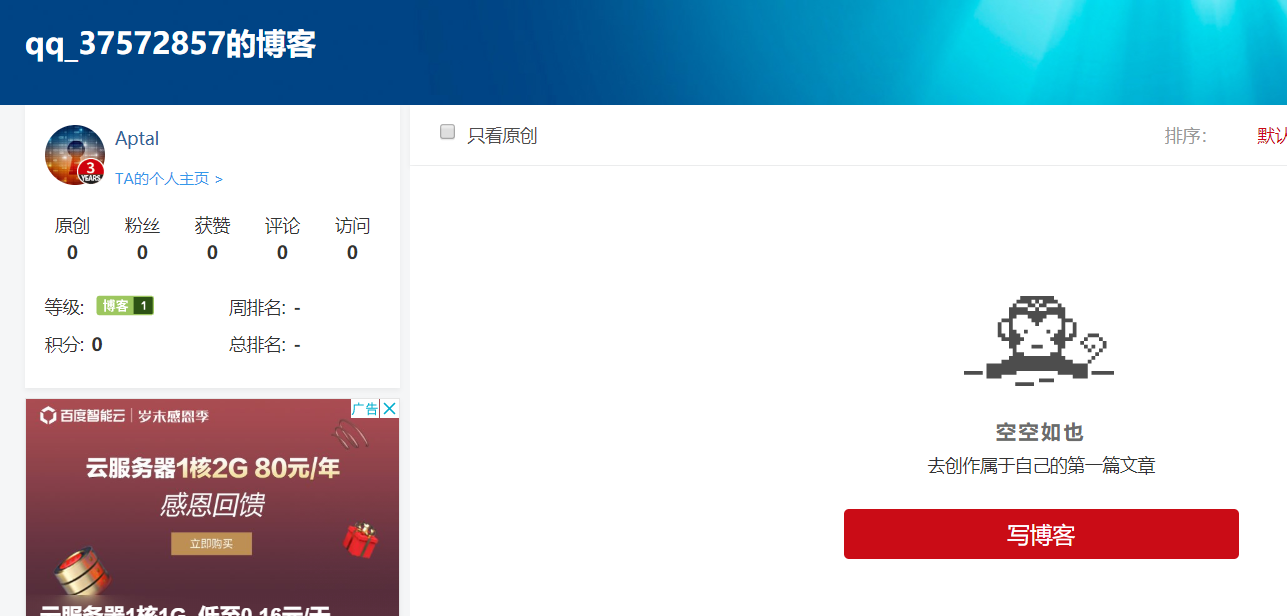
\includegraphics[scale=0.30]{CSDN}
	\caption{CSDN账户}
	\label{fig:CSDN}
\end{figure}

\subsection{博客园账户}
https://www.cnblogs.com/Shy-key/\par
\begin{figure}[h!]
	\centering
	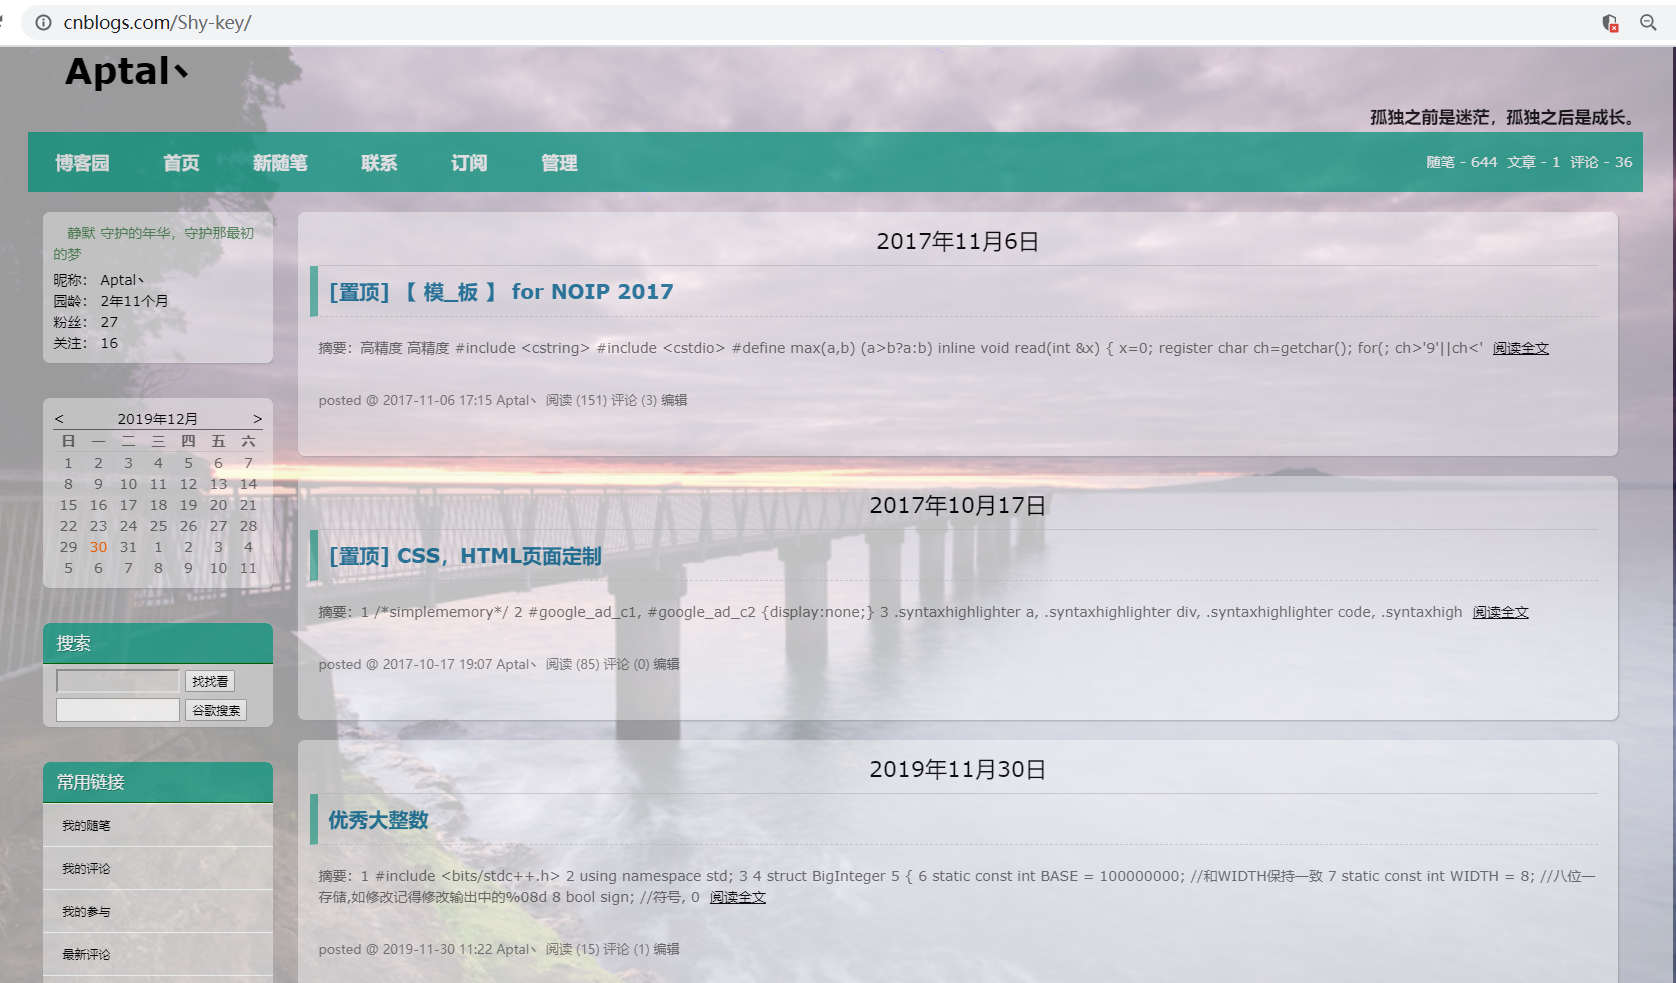
\includegraphics[scale=0.25]{cnblogs}
	\caption{博客园账户}
	\label{fig:cnblogs}
\end{figure}

\subsection{小木虫账户}
http://muchong.com/bbs/space.php?uid=20352795\par
\begin{figure}[h!]
	\centering
	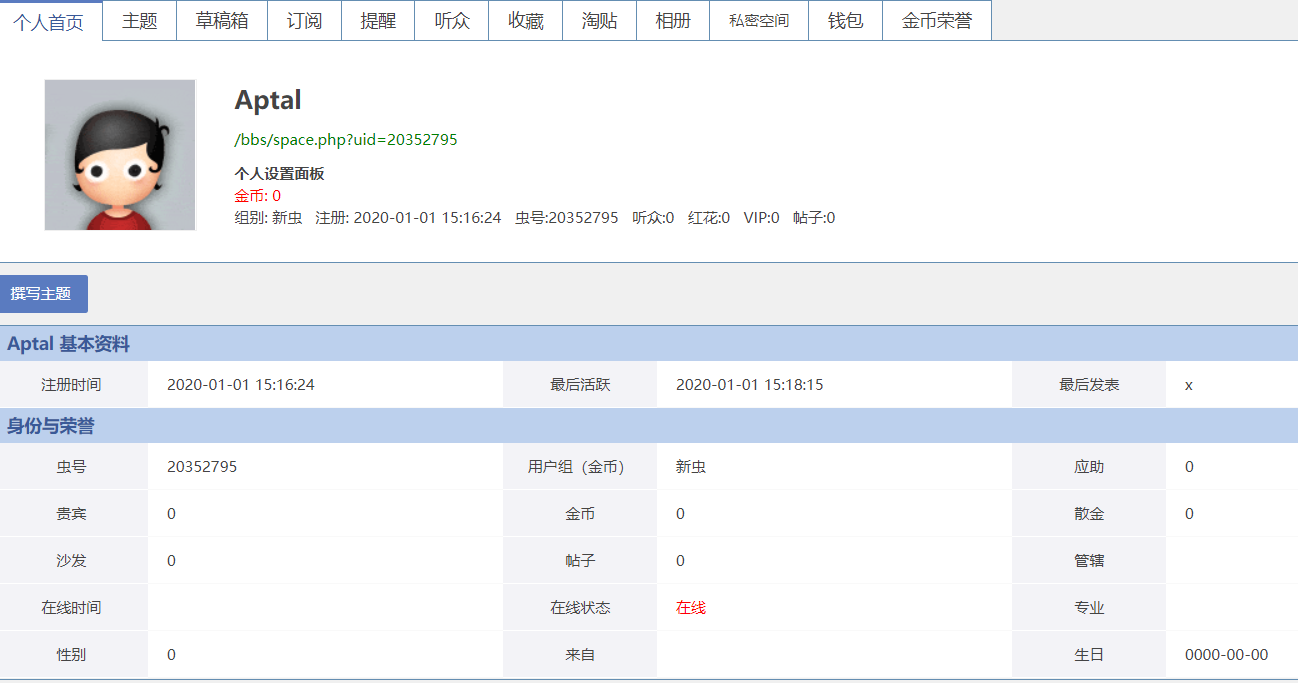
\includegraphics[scale=0.3]{smallchong}
	\caption{小木虫账户}
	\label{fig:smallchong}
\end{figure}

\subsection{观察者账户}
\begin{figure}[h!]
 	\centering
 	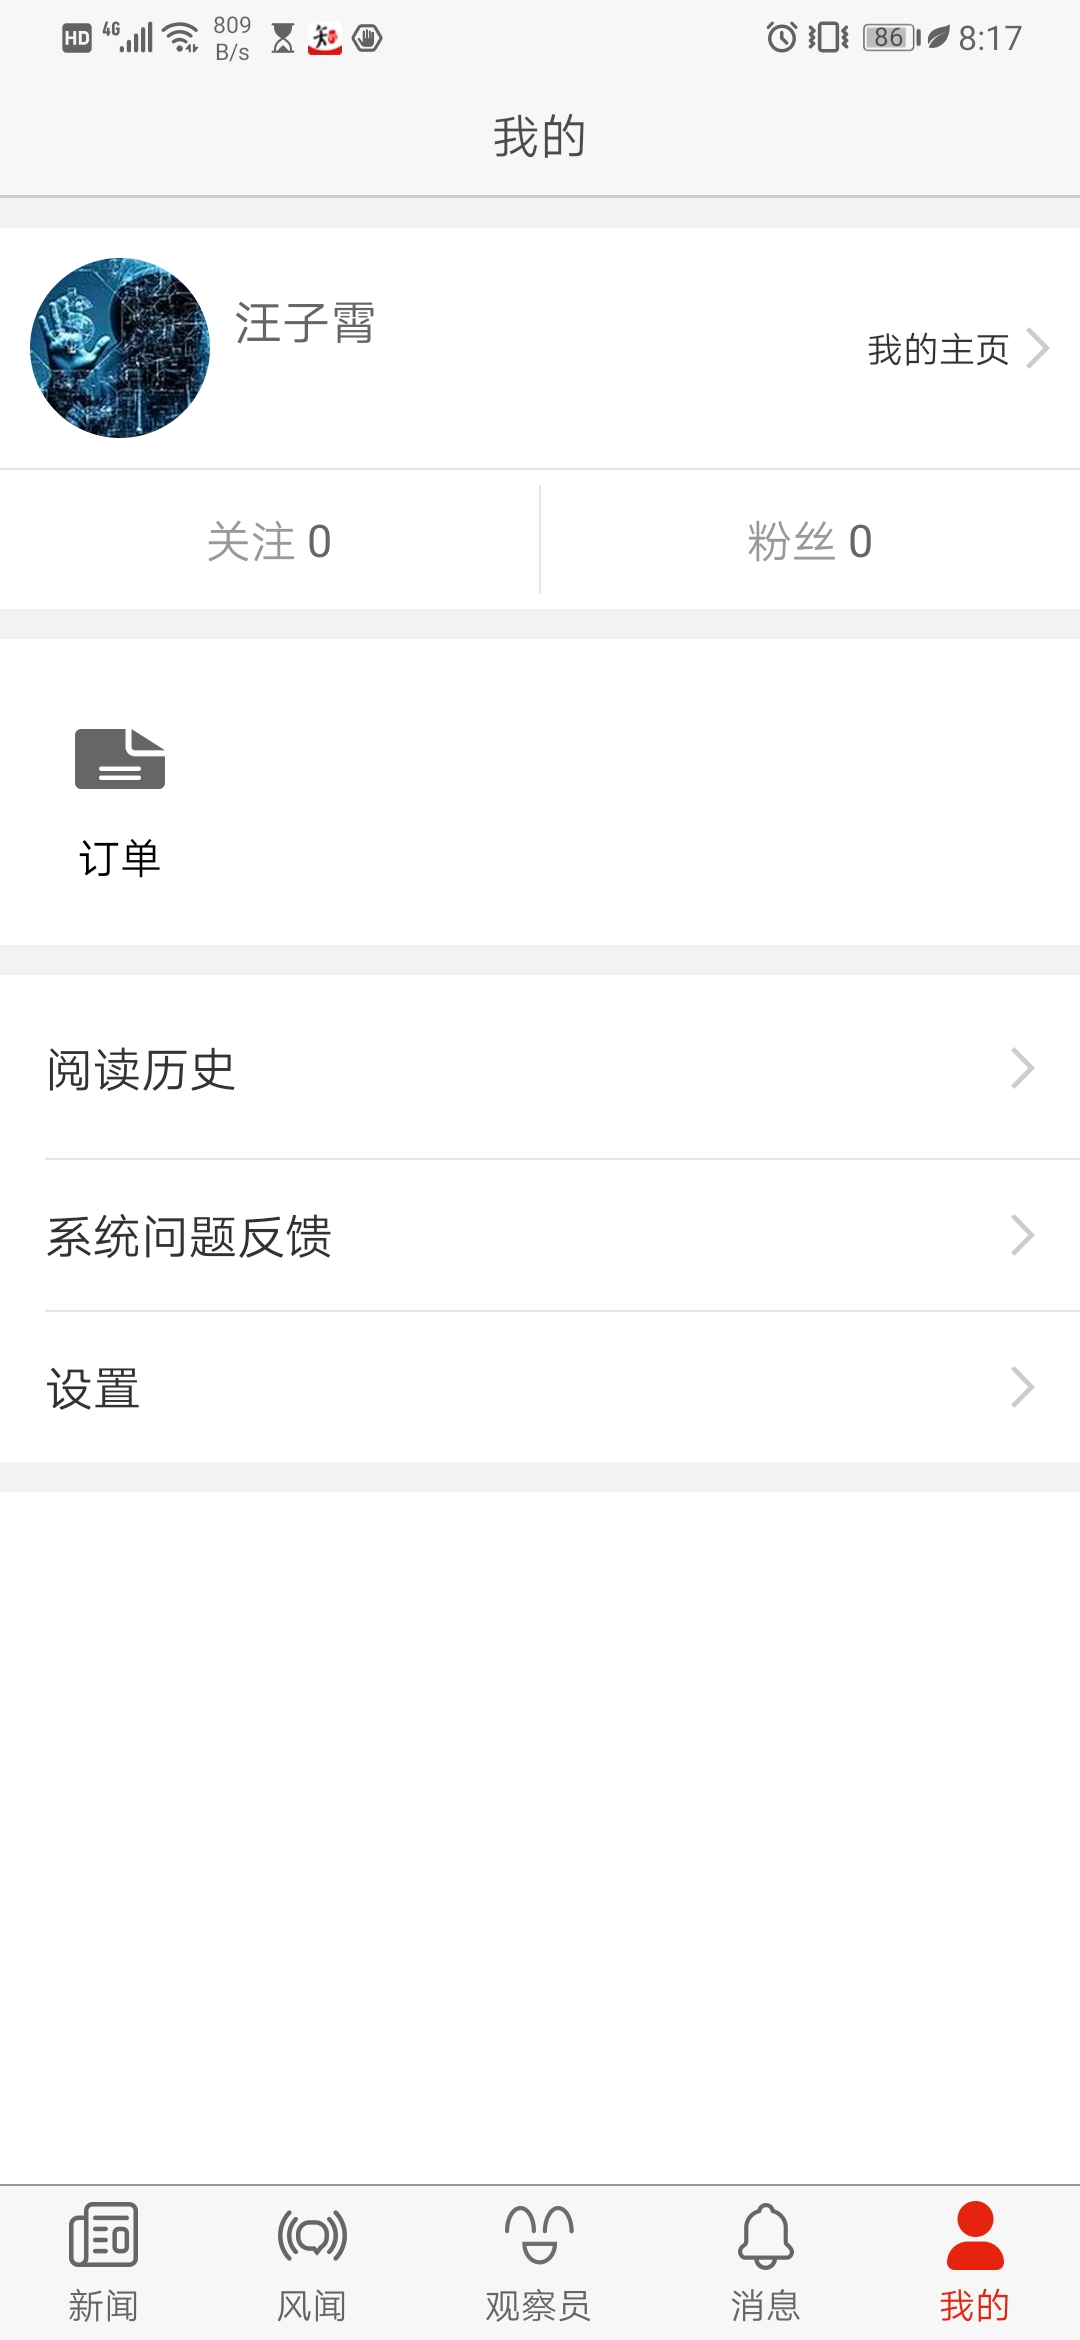
\includegraphics[scale=0.11]{Watcher}
	\caption{观察者}
	\label{fig:Watcher}
\end{figure}
       
\subsection{学习强国}
\begin{figure}[h!]
			  \centering
			  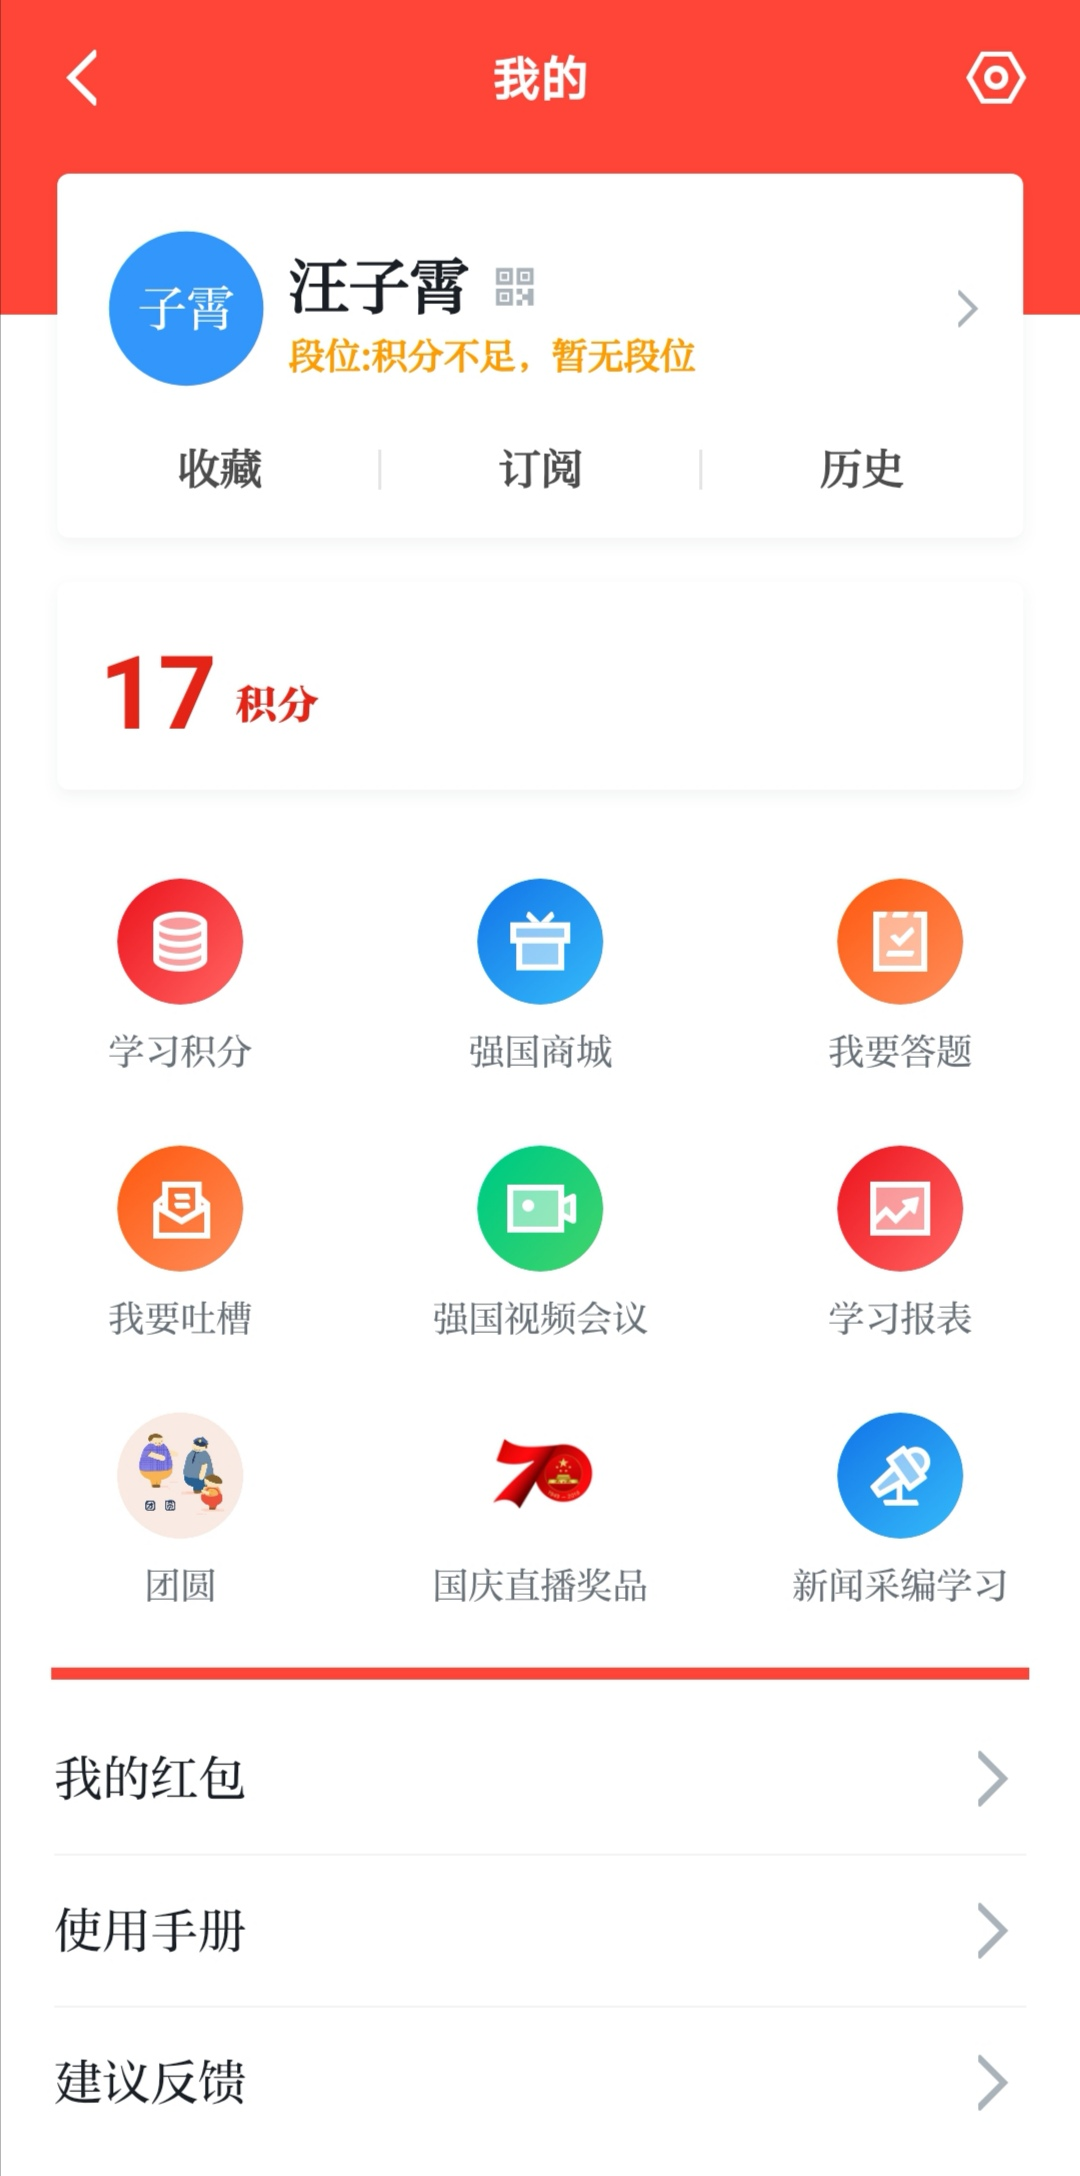
\includegraphics[scale=0.11]{Study_builcounty}
			  \caption{学习强国}
			  \label{fig:Study_builcounty}
		  \end{figure}
\subsection{bilibili账户}
\begin{figure}[h!]
		  	  \centering
		  	  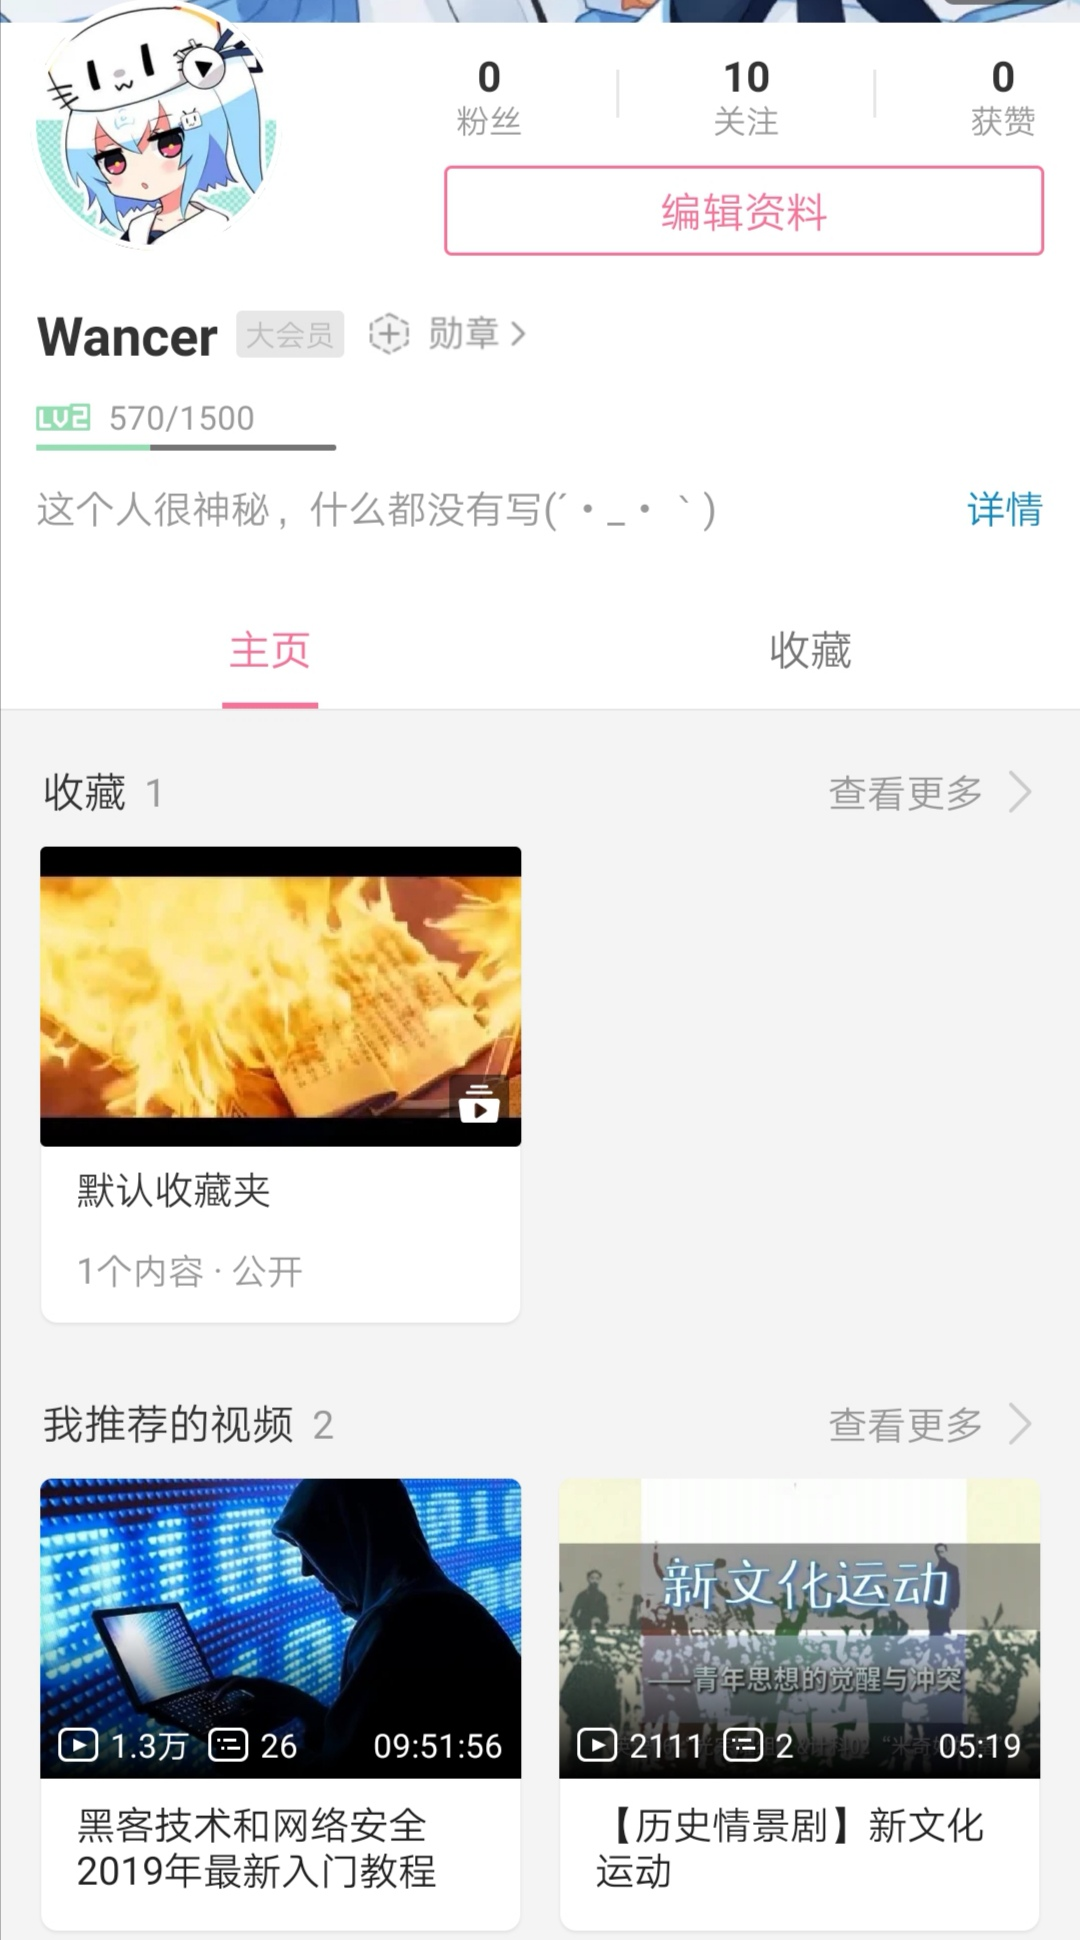
\includegraphics[scale=0.11]{bilibili}
		  	  \caption{哔哩哔哩APP}
		  	  \label{fig:bilibili}
		  \end{figure}

\hspace*{\fill} \\

\bibliographystyle{plain}
\bibliography{references}


\end{document}
